\documentclass[onecolumn,10pt]{IEEEtran}

\usepackage{graphicx}
\usepackage{siunitx}
\usepackage{amsmath,amsfonts,amssymb}
%\usepackage{marginnote} % for editorial use
\usepackage{sidenotes} % for editorial use

\newcommand{\myroot}{../}
\newcommand{\Later}{\textbf{Later.}}
\newcommand{\Calypteanna}{\emph{Calypte anna}}
\newcommand{\Canna}{\emph{C.~anna}}
\newcommand{\MATLAB}{MATLAB}

\usepackage[plain]{fancyref}
\renewcommand{\freffigname}{Fig.}
\renewcommand{\Freffigname}{Fig.} 
\renewcommand{\freftabname}{Table}
\renewcommand{\Freftabname}{Table}
\frefformat{plain}{\fancyrefeqlabelprefix}{(#1)} 
\Frefformat{plain}{\fancyrefeqlabelprefix}{(#1)} 


\title{Autonomous trajectory planning to copysklduvers}
\author{E.~Marcello and D.~Evangelista\thanks{Authors are with the United States Naval Academy, Department of Weapons, Robotics, and Control Engineering}}
\date{today}

\begin{document}
\maketitle

\begin{abstract}
I propose to use a small indoor quadrotor (Crazyflie 2.1) and a multi-camera tracking system (OptiTrack) to attempt to recreate extreme maneuvers observed in flying animals.  My primary goal will be to recreate courtship display dives in Anna's Hummingbirds (\emph{Calypte anna}). In animals, and especially in species with sexual selection / female choice, extreme maneuvers are expected to provide an honest signal of mate quality, e.g. his ability to generate large forces and torques and perform fine control during locomotion, including at high speed. Animals also accomplish these in variable environments with varying flow, turbulence, and lighting conditions. Performing such manuevers with unmanned aerial systems is expected to be an engineering challenge that could help provide robotic systems with access to difficult-to-reach places. I propose a  \SI{24}{week} effort including simulation and proof-of-concept demonstrations in hardware with a total projected cost of \SI{28,470}[\$] including a cost of \SI{370}[\$] in new materials. 

%This research proposal seeks to use aggressive quadrotor maneuvering and path planning to fly the same trajectory Anna’s hummingbirds execute during their courtship display dives with a Crazyflie 2.1 quadrotor. Aggressive autonomous maneuvering for quadrotors has been a focused area of study by many researchers over the past several years; however, there have not yet been many attempts at replicating aggressive flight patterns seen in biological species. In being one of the first research topics into flying Anna’s hummingbird dive trajectories with an autonomous platform, this paper aims to discover an advantage to this specific type of maneuver for autonomous aerial vehicles. To execute this task, I will be relying heavily on prior work completed in autonomous control of the Crazyflie quadrotor, utilizing a quaternion model of the quadrotor flight dynamics. Additionally, I will be using previously obtained data for the Anna’s hummingbird flight trajectories. To measure the feasibility of the maneuver I plan to conduct trials both in simulation and in proof of concept demonstration that will compare the trajectory of the quadrotor to the hummingbird flight trajectory using a root mean square error between sampled data points along the trajectory paths. The total projected cost of the project is \SI{28470}[\$] including a cost \SI{370}[\$] in new materials. The timeline estimates project completion in 24 weeks, with the highest risk being my requirement of learning 2 new programming languages, ROS and Python, and possible damage to the Crazyflie quadrotor in the event of a failed maneuver
\end{abstract}

\begin{IEEEkeywords}
capstone, robotics, controls
\end{IEEEkeywords}

\section{Background and motivation}
\IEEEPARstart{A}{nimals moving in a real environment} face many challenges that are currently unsurmountable for typical engineered devices, including small size, difficult-to-achieve power-to-weight ratios, ability to operate in multiple environments, and the ability to control complex maneuvers even in the presence of environmental disturbances such as wind, water flow, or turbulence, variable lighting, or even attack from predators or conspecific rivals. These alone make them worthy of engineering study, but such interdisciplinary work is not a one-way street. 

Biologists may also wish to use engineering to learn how an organism does what it does.  As an example, consider the aerodynamic principles of ``helicopter'' samara seeds such as in maples (\emph{Acer sp.}) and convergently evolved in many other groups.  Samaras are able to slow their descent to the group using a spanwise asymmetric weight distribution and wing structure to facilitate autorotation, allowing them longer hang time during which, on rare occasions, they are swept quite far by a lucky gust of wind. The resulting long dispersal distances are quite advantageous for the saplings, who no longer have to compete with the mother tree. The study of the first autorotating seeds in the fossil record made heavy use of engineering techniques such as autorotation theory, consideration of stability from the vertical separation of the center of gravity and the center of pressure, and nondimensional coefficients governing flight \cite{stevenson2015when}.  As for applications\footnote{We emphatically believe applications of basic biomechanics research may not be immediately obvious but that this is not a reason to ignore biomechanical systems of interest.}, researchers in \cite{who2019maple} developed a monocopter based off of this concept, and were able to develop control algorithms for actively steering such a device. 

Robotic systems are potentially a way to examine form and function in organisms, and organisms are potentially a source of inspiration for improving the robots.  In \cite{feltman2014creepy}, sidewinder-type locomotion, observed in all snakes but most characteristic of the sidewinder rattlesnake (\emph{Crotales cerastes}), was studied by creating a robot to imitate it. In sidewinder locomotion, snakes move across granular media like hot desert sand in a direction lateral to their main body axis; this is accomplished using a combination of body twisting and bending to create moving points of contact with the ground as the body bends.  The robot was developed like a snake, and was programmed to copy as closely as possible the movement of the sidewinder. The initial test had success on level ground, but no such luck on steeper slopes. On closer observation of the live snake, it was discovered that the sidewinder used two independent wavelike motions to move instead of just a single wave. Once this was implemented in the robot, the robot was able to navigate just like the sidewinder, and a new form of ground travel was made attainable by robotic machines. This discovery has applications of movement over a variety of different terrain that a typical wheeled robot would not be able to navigate.

I will be attempting to enhance a quadrotor’s maneuverability by studying the flight patterns and maneuvers of Anna’s Hummingbirds (\Calypteanna), a \SI{5}{\gram} hummingbird native to western North America. Male Anna's Hummingbirds perform a display dive in order to win matings with choosy females. The dive reaches speeds above \SI{20}{\meter\per\second} \cite{larimer1995accelerational} and ends with a 9G pullout maneuver (full 3D field kinematics determined in \cite{clark2009courtship}) culminating in a display of red iridescent feathers on his gorget (throat) and a high frequency tweeting noise made by flow-induced vibration of the distal two retrices (outer tail feathers) \cite{clark2008annas}. Such a maneuver would normally cause G-induced loss of consciousness in a human pilot without a g-suit.  The difficulty of the manuever makes it an honest signal \cite{zahavi1975mate} of mate quality to Anna's Hummingbird females as it requires skill and power to complete. Thus, it is expected to be difficult for a \SI{19}{\gram} quadrotor\footnote{The Crazyflie 2.1 mass is approximately the same as the largest living hummingbird species, the Giant Hummingbird (\emph{Patagona gigas}), native to the Andes.}  to imitate and a worthy challenge. I intend to discover how feasible the dive maneuvers actually are for quadrotors, and explore their operational limits in this respect. 

Unmanned aerial systems are becoming increasingly more autonomous for tasks with position control at comparatively low speeds; a guiding research question is how extreme maneuverability can augment their capabilities by building on previous work in quadrotor control  \cite{mellinger2011minimum, greiff2017modelling}.  The applications of this research are twofold: it will both help in developing a greater understanding of the physical limitations of extreme maneuverability on quadrotors (engineering problem), and it will also provide a greater idea of the effects of such maneuvers on flying animals. The ability to automate the hummingbird dive maneuvers means that other forms of extreme maneuvers might also be autonomously executed, perhaps providing a toolbox or set of ``riffs/licks'' to use when a UAS is presented with a maneuvering challenge during a mission.  If combined with enhanced sensing abilities, autonomous MAVs would be able to navigate through obstacle-heavy environments with greater speed and ease, allow for evasion or penetration/infiltration, or simplify recovery. 

In addition to this, a successful device could be used in behavioral playback studies in which live hummingbirds are presented with a controllable stimulus mimicking the male display dive.  If a quadrotor were to execute this dive for a female Anna's Hummingbird, could the quadrotor generate a favorable response from her? If so, it may be possible to alter the pattern to present a super-normal stimulus or probe which aspects of the display are most appealing to her.  Such a study in hummingbirds would be novel\footnote{von Frisch, Lorenz, and Tinbergen won the 1973 Nobel Prize for Physiology or Medicine for ``discoveries concerning organization and elicitation of individual and social behaviour patterns...'' among other things, including use of robots to examine honeybee dance language and supernormal stimuli in herring hull beak markings.}  as biologists have not been able to produce the maneuvers themselves.






\section{Problem statement}
I aim to replicate the display dives of male Anna’s Hummingbirds (\Calypteanna) with an autonomous quadrotor platform. 

My project assumes the following are provided: a quadrotor and  flight controller (e.g. Crazyflie 2.1, Bitcraze, Malm\"{o}, Sweden), and a method of obtaining three-dimensional (3D) position data of the quadrotor in test flights (e.g. OptiTrack, NaturalPoint Inc., Corvalis, OR). Example trajectories obtained from live hummingbirds will be obtained from \cite{clark2009courtship}.  Given a desired hummingbird flight trajectory, depicted in \fref{fig:problem-statement-1}a, the system will autonomously generate and execute the control inputs required to successfully complete the maneuver. 

A successful maneuver is defined as a root mean square error calculation of less than \SI{5}{\percent} between the time-scaled hummingbird trajectory and the quadrotor trajectory, where each trajectory is defined as a matrix array of positions in the $x$, $y$, $z$ right handed coordinate frame with a given sample period, $\delta t$. The hummingbird trajectory will be scaled by a constant factor in time to allow for the physical limitations of the quadrotor -- e.g. the quadrotor may only have to travel the desired trajectory at half the speed of the hummingbird to still achieve a successful maneuver. This is a necessary adaptation due to the impressive speed and acceleration capabilities of the Anna’s hummingbirds relative to their size \cite{clark2009courtship}. The ideal result is to fly the hummingbird trajectory at the same speed as the hummingbird, but this may prove to be impossible due to the physical constraints of the quadrotor and lab space in Maury 201.
\begin{figure}[h]
\begin{center}
\includegraphics[height=1.88in]{\myroot/figures/problem-statement-1a.png}%
\includegraphics[height=1.88in]{\myroot/figures/problem-statement-1b.png}
\end{center}
\caption{(a) The five stages of an Anna’s Hummingbird dive maneuver, from \cite{clark2009courtship}. (b) A quadrotor using path planning to fly through a thrown hoop, from \cite{mellinger2011minimum}.}
\label{fig:problem-statement-1}
\end{figure}

As a stretch goal, I will also analyze and replicate a variety of different types of hummingbird dives and maneuvers, to include evasive aerial maneuvers \cite{sholtis2015field, cheng2016flight}. Success will be determined in the same fashion as described above.





\section{Literature review}
%The inspiration of this project proposal has its roots in the high maneuverability seen by hummingbirds. As such, it was essential to be able to gather data on hummingbird trajectories in order to study their feasibility of being replicated by a quadrotor. There have been many bio researchers that have delved into the study of hummingbirds, however I will mainly discuss the works \cite{clark2009courtship} and \cite{cheng2016flight}. 

The work in \cite{cheng2016flight} determined the trajectory and body kinematics of four different hummingbird species in an evasive maneuver. This was done by startling the birds while they were hovering, and observing their movements with three high definition cameras to provide a 3D position \cite{hedrick2008software, theriault2014protocol, jackson20163d}. Birds were marked with water-soluble white paint to ease digitization and tracking. I will use a similar optical tracking methods as in \cite{cheng2016flight, hedrick2008software, theriault2014protocol, jackson20163d}, with the added simplifications of being able to install known, infrared (IR) relfective markers for automatic tracking and using a RANSAC algorithm to estimate pose. In addition, the evasive maneuvers studied in \cite{cheng2016flight, sholtis2015field} could be useful for quadrotors attempting to avoid capture or a counter-UAS drone denial system (e.g. USNA Project Midknight or similar).

% Water-soluble white paint was used to make dot markings on the hummingbird’s body to help model the wing and head positions for each trial. The data they acquired in their experiments includes many more details than I will need to use, however they provide data on the hummingbird’s velocity and trajectories for several trials which I can use to help develop my quadrotor trajectories. , they and I will both be using optical data to obtain a position fix. With regard to the type of maneuver that these birds are required to perform, it aligns well with the type of experimentation that I aim to work with. Evasive maneuvers are certainly a type of extreme maneuver, and these patterns may prove to be something that I wish to try on my quadrotor. Evasive maneuvers can be useful for quadrotors if they are in threat of being netted, and if I am able to copy the hummingbird’s trajectory, further analysis and testing may prove that this type of trajectory provides a maneuvering or sensing advantage to the quadrotor in evasive flight.

The work in \cite{clark2009courtship} obtained fully 3D field kinematics of courtship dives in \Canna\ in order to study extreme locomotor performance in animals. \cite{clark2009courtship} used multiple calibrated high speed cameras and manual digitization to reconstruct the birds' 3D position during dives.  Splines were used to estimate acceleration and velocity from positions without undue amplification of noise. \cite{clark2009courtship} also examined wing and tail movements and sounds produced during dives.  As a measure of the biomechanical difficulty of the maneuver, \cite{clark2009courtship} estimated the maximum stresses in the humerus during dive pullout; such a quantity would be extraordinarily difficult to measure \emph{in vivo} but in  my work there is a possibility of directly instrumenting the quadrotor to examine forces, torques, stresses, and engineering limits. 
%Again, this is more detailed data than I will need for trajectory replication on my quadrotor. This paper gives an insight into what exactly I will be trying to achieve through the extreme maneuverability of my quadrotor. Since this type of maneuver is estimated to cause a lot of strain on the hummingbird, it is likely to also cause a lot of strain on a quadrotor. Through simulation and proof of concept demonstration, I will be able to provide a more accurate picture of just how difficult these maneuvers can actually be.

After obtaining these hummingbird trajectories, an effective method of modeling a quadrotor and conducting trajectory planning is required. In \cite{tomic2014learning}, the authors developed metrics and constraints for quadrotor maneuvering performance and a machine learning workflow. This was achieved through the solving of an optimal control problem offline, and then using a machine learning technique to learn these trajectory solutions with the given constraints. The result was then used to develop online solutions  for near-optimal trajectories for a quadrotor. This was done in the $x$-$z$ plane for point to point and perching maneuvers, as well as joint trajectories. To validate their solution, they flew these optimal trajectories using both Simulink simulations, and proof of concept demonstrations. Since I will be using a quadrotor platform, this paper directly applies to my problem statement as a good reference base that I can use to springboard my exploration into more complex extreme maneuvering. The basis of this work will give me a much more quantitative measure of success in terms of how close my developed trajectories are to an optimal path. \cite{tomic2014learning} is very thorough and provides a clear distinction and improvement on previous work in quadcopter trajectories, especially with regard to the joint trajectory problem. I can build on this by expanding into 3D trajectories instead of just working in a 2D plane, and I can also try to utilize their proxy-based joining method to create a desired path curvature.

In \cite{sabatino2015quadrotor}, the authors developed a linearized model of a quadrotor in planar motion. The careful process by which the quadrotor dynamics are identified and modeled will be helpful in my own research as I develop my own model for the quadrotor that I will be using. In \cite{sabatino2015quadrotor}, their modeling method is done for three different linearization methods and each of these is compared to each other by running a Simulink simulation with each controller. Quantities compared include several attributes of the step response, and the actual trajectory of the quadrotor compared to the desired trajectory. This comparison method between the different trajectories is similar to the validation work that I will need to do on my own simulation. As such, this work will help me to better understand ways of determining the accuracy of my trajectory testing in simulation, and in proof of concept demonstration. This paper, while a good starting point for my work, does not attempt to go into more complex maneuvers. These are discussed in greater detail in the following works.

In \cite{liu2017planning}, the development of trajectories and path planning for UAVs was accomplished. They did this by determining the maximum overload, minimum turn radius, and maximum flight endurance of the experimental quadrotors in order to come up with feasible aggressive trajectories. Trajectories had the constraint that they had to follow a sixth order (or lower) polynomial trajectory. Much like my proposed concept, this work develops an attitude and trajectory controller with appropriate initial and final conditions, as well as a boundary “tube” which the quadrotor must stay within for every trajectory. The work in this project is heavily relevant to my proposed work, as they achieve a working simulation of aggressive trajectories with their path-planning algorithm and onboard controllers. I would like to expand on this work by flying a shorter trial with hummingbird-like flight patterns. 

Finally, \cite{mellinger2011minimum} offers some of the closest work to exactly what I am proposing for my own work. The main focus of this paper is to create trajectories for quadrotors in real time in an indoor or constrained environment. They also pay particular attention to the velocity and acceleration vectors of the quadrotor throughout its maneuver. I will also need to be able to achieve these types of measurements from my system, and be able to change my controller to affect them in an appropriate manner in order to fully achieve a trajectory flight path that replicates a hummingbird maneuver. \cite{mellinger2011minimum} also uses temporal scaling to fly their trajectories at different speeds, which is exactly what I will need to do when and if I find that flying the hummingbird trajectory at full speed is either not possible or extremely dangerous. 





\section{Demonstration Plan}
To demonstrate the objective of replicating \Canna\ display dives,  I will simulate the system in \MATLAB\ and Simulink.  This will be followed up with a proof-of-concept demonstration, provided I am able to achieve successful trials in simulation first. The simulation will be more general and will allow easy changing of parameters and control methods to more completely explore the space; simulations will also allow examination of behavior at actual hummingbird flight speeds. Simulations, by necessity, make simplifying assumptions, so actual testing and demonstration using real quadrotors is also planned.  
% This part is way too wordy and non-sequitur. 
%Before I describe these processes, it is important to mention why these are the methods I chose to implement. A simulation is general in that I can run the simulation for many iterations to see how the controller will react to different input parameters. The input parameters themselves are very specific; however, the ability to change parameter values will allow me to assess the full capabilities of the quadrotor system to determine if I can eliminate the need to do a time-scaled comparison to the hummingbird trajectory. The simulation will be coded using MATLAB and Simulink, both are software with which I have the most experience in creating simulations. My simulation code will be made available after the completion to this project on Git for those wishing to replicate my simulated results. Unfortunately, the realism of this simulation is limited, and as a result I will have to do a proof-of-concept demonstration to truly prove the ability of the quadrotor. Being a much more specific process, it will likely vary slightly from the simulation results, and need to be tweaked based on the level of success seen in the first few trials. Ultimately, the proof-of-concept demonstration is an essential piece to this research since a simulation doesn’t have any real world application except in principle. The experiment will enlist the use of a Crazyflie quadrotor platform, and an OptiTrack motion capture system in order to gather position vs. time data. This will help ensure accuracy in the quadrotor’s trajectory and as such, provide a higher level of confidence in the experiment’s success.

For my concept demonstrations, I will be modeling the rigid body dynamics of the quadrotor using the quaternion model in \cite{greiff2017modeling}. A quaternion is defined as 
\begin{equation}
Q = a + b i + c j + d k
\end{equation}
where $i$, $j$, and $k$ are imaginary unit vectors. This model also assumes a right-handed coordinate system where $i\cdot j = k$ , and the fundamental assumptions hold true -- i.e.  $i^2 = j^2 = k^2 = ijk = -1$.  I have chosen to use this model due to the limitations of the Euler model at high rotation angles. The quaternion model will be robust to these extreme angles, and is therefore better suited for my experiment. \emph{\textbf{Evangelista comment here: this is sort of strange to mention here. It's like saying I plan to use math, or matrices, or eigenvalues. Choosing to represent rotations as quaternions is a useful thing for avoiding gimbal lock associated with singularities in the Euler angle representation, but would not be considered a defining characteristic of what you plan to do, more like a low level design choice comparable to what units you use, or if you like floats or doubles.}}




\subsection{Simulation}
To create a feasible simulation for this research, I will model the Crazyflie quadrotor platform to be used in simulation. This involves determining the various thrust vectors of the motors, and the calculation of many performance metrics. Thankfully, much of this work has already been done, and I will be relying heavily on the work in \cite{cheng2016flight} to create a useful model for the quadrotor in \MATLAB\ and Simulink. Due to the extreme maneuvering of the quadrotor, I have chosen to use a quaternion coordinate system to describe its position, for flight control purposes only. The trajectory comparison will be conducted in the $x$, $y$, $z$ Cartesian coordinate frame. A quaternion is defined as a vector of one real and three imaginary vector directions, $i$, $j$, and $k$. Once this has been accomplished, I will obtain and upload Anna’s Hummingbird flight trajectories into \MATLAB. These will serve as truth, or the desired trajectories for my simulation to attempt to run through. Once this is complete, I will develop, or obtain from another source, a path-planning flight controller algorithm that is able to take in a desired flight path and create an appropriate response to fly this desired flight path with minimal error. The feedback diagram of this control concept is shown below in \fref{fig:demonstration-2}. In principle, a desired trajectory will be developed from a path-planning algorithm that takes in the time scaled hummingbird trajectory and calculates the idealized pitch and motor torque and speed at each time step in order to fit this trajectory with as little error as possible. This signal will be combined with some sort of inertial measurement true position feedback to produce the error signal to the onboard flight controller. The flight controller will send a signal to the motors on the quadrotor based on this error signal to come as close as possible to zero error for the next time step, and the cycle will repeat until the quadrotor has completed its maneuver. My simulation will replicate this decision-making process using numerical integration to obtain the position data for every iteration.
\begin{figure}
\begin{center}
\includegraphics[width=\columnwidth]{\myroot/figures/demonstration-2.png}
\end{center}
\caption{Functional Block Diagram of the controller feedback loop. \emph{\textbf{Evangelista comment: not sure what is shown here. There's an IMU related loop onboard the vehicle, and an outer loop driven by the OptiTrack and your controller offboard; I only see the inner loop here.}}}
\label{fig:demonstration-2}
\end{figure}

Finally, to determine accuracy of the trial I will compare the actual flight path of the quadrotor with the desired flight path, and determine a time-scaled root mean square error between the two position vs time datasets. This error will be calculated using \fref{eq:demonstration-1} below:
\begin{equation}
e(t) = \sqrt{
\begin{bmatrix}
x(t) \\ y(t) \\ z(t)
\end{bmatrix}_a^2 
-
\begin{bmatrix}
x(t) \\ y(t) \\ z(t)
\end{bmatrix}_d^2
}
\label{eq:demonstration-1}
\end{equation}
where $e(t)$ is the error at a specific time step in the trajectory, all operators are considered element-by-element matrix operations, and the subscripts $a$ and $d$ represent the actual traveled trajectory and the desired trajectory respectively. The error for every time step will be averaged together to determine the root mean square error of the data in the form of a \num{3x1} matrix. The magnitude of this matrix will be the official value for the root mean square error. Without any other indications, a successful trial will be considered a root mean square error of less than ten centimeters over the entire trajectory. Since the hummingbird trajectory is time-scaled—down to only a fraction of its true speed—the quadrotor will be responsible for marking every position at the time it is supposed to be located at that position, therefore removing motor operation constraints as a possible source of error.

If I am able to accomplish a working simulation with the Anna’s Hummingbird courtship dive maneuver, I will try to make the simulation slightly more general so it can apply to a wide variety of hummingbird dives and maneuvers. This can include evasive maneuvers, and potentially other types of stunts.






\subsection{Experimental work}
	Provided that the simulation is able to achieve several successful runs, a proof of concept demonstration will be deemed necessary for further analysis into the possibility of actually autonomously flying a drone through hummingbird flight trajectories. The hardware components necessary for this experiment include a fully functional Crazyflie quadrotor (Bitcraze, Malm\"{o}, Sweden), and an OptiTrack system (NaturalPoint Inc., Corvallis, OR). The quadrotor will be the object of the experiment, and the OptiTrack system is a highly accurate way to obtain position data for the Crazyflie in flight using visual information from nearly 20 cameras staged around the outside of the testing area. Experimentation will be conducted indoors for the initial trials to minimize any aerodynamic noise \emph{\textbf{(Evangelista comment: but being able to do this in noise is of interest?)}}. There is a distant possibility to moving into an outdoor environment if early testing shows signs of having promising results. I will need several batteries for the Crazyflie to ensure sufficient trial and testing periods, and I will also need to attach approximately five OptiTrack visual markers on the Crazyflie drone to ensure that it is able to be detected by the OptiTrack system. These marker additions will be taken into account in simulation first in order to ensure readiness to counteract any effect they may have on the dynamics of the quadrotor in the feedback loop.
	
The first step to demonstration will involve the conversion of coding language from \MATLAB, used for the simulation, to Python\footnote{Evangelista comment: why not start in Python?}. Python will be used to implement the path-planning control algorithm on the Crazyflie. To fly the trajectory, the quadrotor system will follow the feedback loop portrayed in \fref{fig:demonstration-2} above. When the quadrotor is ready to fly the trajectory, the OptiTrack system will obtain the position vs. time information of the Crazyflie using visual sensor data, accurate to $\approx \SI{1}{\milli\meter}$. This data will be compared to the desired hummingbird trajectory in post-processing to determine the flight accuracy, just as in the simulation.

%\subsection{Property measurement}
\subsection{Technical risks and mitigation}
It is possible that the Crazyflie quadrotor will crash during experimental testing. The risks to damage on the quadrotor will be mitigated by 3D printing propeller guards to prevent hardware damage on unintended impact.

\emph{\textbf{Here refer to Canlas 2019 experience. Canlas has been attempting to fly patterns using legacy Crazyflie 2.0 hardware. He has been plagued by the cumulative damage that happens each time a device takes a hard landing. Mitigate in two potential ways: early obtaining replacement hardware and potential to switch to an alternate platform (DJI Tello) as used by Cuniff (2019) and potentially by Credle (2020). }}

\subsection{Time risks and mitigation}
Learning ROS will be the most time-intensive part of this project, as well as finding/developing  a suitable control algorithim that will allow my quadrotor to fly the necessary trajectories. 

\emph{\textbf{This is the first mention of ROS. Also, ROS is very slow most useful for the slow position path planning autonomy that you dumped on in your intro. It is not expected to be fast enough for the most dynamic maneuvers?}}

\subsection{Justification of high risk activities}
In order for this research to be conducted successfully, I will likely need to learn ROS programming language, and re-familiarize myself with Linux shell. This will likely delay work for \numrange{1}{3} months while I learn these new computer languages; however it is a necessary step in making full use of the Crazyflie developmental platform, and being able to communicate between it and the OptiTrack system.

\subsection{Budget}
\emph{\textbf{Please add the following disclaimer: ``Labor and overhead costs are estimated only for EW502 training purposes and do not actually reflect real costs that would be supported by project sponsors.''}}

\emph{\textbf{Your budget as presented in your pitch and proposal ought to give some indication what you are considering as in stock versus new items. For example, you plan to leverage the presence of OptiTrack system and of gear from what Canlas has leftover, and from School of Drones. You are getting some new stuff ahead of time but probably (given risk mitigation) ought to put in to get more in future as you break more stuff. There is no incentive here to make this look small - make it look realistic so I can use it to find more money to buy stuff and maybe explicitly add 20-50\% margin too. }}

\begin{table}[hb]
\caption{Budget}
\label{table-budget}
\end{table}

I will be purchasing a new Crazyflie 2.1 since many of the Crazyflies that we own have been crashed multiple times and have potentially lost functionality I will need for my highly precise and aggressive maneuvering.




\section{Conclusion}
The proposed research discussed in this paper is concerned with the replication of the highly aggressive aerial maneuvers of the Anna’s Hummingbird on an autonomous quadrotor platform. Specifically, this research aims to determine the extent to which these maneuvers are possible through analysis of a time-scaled root mean square error between the bird and quadrotor trajectories. Analysis will be conducted through both simulation and proof of concept demonstrations on the Crazyflie 2.1 platform. The proof of concept demonstration will utilize an OptiTrack motion capture system to ensure a high degree of accuracy is recorded for the quadrotor trajectory, and the experiment will be conducted inside to minimize any possible disturbances in the air. \emph{\textbf{This paragraph is good, punchy. Make your abstract look more like this?}}

Novelty: This research is the first attempt to autonomously mimic a hummingbird dive trajectory, and it has promise in being successful at developing a greater understanding of the limits of extreme maneuverability in our currently utilized UAV quadrotors. The biggest risk to the project’s completion is my understanding of ROS and Python programming languages. Lapses in my understanding could cause my research timeline to drag out longer than intended, and as a result could possibly inhibit my ability to draw any significant conclusions about the quadrotor’s capability in executing these extreme maneuvers.

\section*{Acknowledgements}
\Later

\bibliographystyle{IEEEtran}
\bibliography{IEEEabrv,\myroot/references/marcello}





\appendix
\section{Timeline}
\emph{\textbf{Remember to include in your timeline things like Army-Navy game, holidays, weddings, Christmas, Spring Break, the trip you and your buddies want to take, etc. and to build into it margin to the right so that you finish enough in advance of Capstone Day in April.}}

\begin{enumerate}
\item \textbf{Add Item 0. Get turnover from Canlas, Cuniff, exercise stuff to know we can fly, can talk to optitrack, and that you have a laptop available with all software planned to be used.}

\item Simulation
\begin{enumerate}
\item Familiarize myself with simulation capabilities.
\begin{enumerate}
\item Test all demos (1 week)
 \item Adapt some variables to see how the simulated results respond (1 week)
\item Upload model of the Crazyflie quadrotor to the simulation to be used for accurate simulation data. (1-3 days) 
\end{enumerate}

\item Create a desired path for the Crazyflies to fly.
\begin{enumerate}
\item Choose 3 different desired flight shapes and adapt simulation code to take them in as the desired flight path for the quadrotor. (1 week)
\item Run simulation tests and error calculations. Debug any issues with simulation. (1-2 weeks)
\item Plot all position, velocity, and accelerations vs. time (both linear and rotational on all 3 axis). (1-2 days)
\end{enumerate}

\item Test hummingbird trajectories in simulation.
\begin{enumerate}
\item Upload hummingbird dive trajectories into simulation. (3 days)
 \item Run simulation and plot position, velocity, and acceleration data vs. time for all 3 axes in both the linear and rotational frames. (2 days)
\item Conduct error calculations between the desired trajectory and the simulated trajectory of the quadrotor. (1 week)
\item Determine acceptable region of error, and determine a maximum theoretical performance for the quadrotor as a measure of how fast the quadrotor is able to complete the maneuver as compared to the hummingbird. (1 week)
\end{enumerate}
\end{enumerate}
 
\item Proof of Concept Demonstration
\begin{enumerate}
\item Purchase new Crazyflie and supporting materials
\begin{enumerate}
\item Create online shopping cart pdf of all materials: Crazyflie, extra blades, extra battery, more OptiTrack markers, etc. (3 days)
\item Create RQ forms and ITPR forms (\textbf{Marcello}\footnote{I've done the first ones as examples for you. You're doing all the others.}) (1 week).
\end{enumerate}

\item Obtain manual control of a Crazyflie with remote control.
\begin{enumerate}
\item Configure Crazyradio and obtain positive connection to the Crazyflie using Crazyflie PC client software. (1-2 days)
\item Connect controller to laptop and configure manual controls to Mode 2 (1 day)
\item Conduct takeoff/landing procedures. (1 day)
\item Fly a rough 3D pattern using manual control. (1 day)
\end{enumerate}

\item Obtain flight data using OptiTrack
\begin{enumerate}
\item Set up OptiTrack system to recognize Crazyflie as a rigid body. (3 days)
\item Run sample code to log flight data. (3 days)
\item Manually fly the Crazyflie and obtain flight data. (3 days)
\item Plot position, velocity, and acceleration data vs. time for all 3 axes in both the linear and rotational frames in \MATLAB. (3 days)
\end{enumerate}

\item Fly the Crazyflie Autonomously
\begin{enumerate}
\item Read about ROS and develop python proficiency (4 months, concurrent)
\item Develop/Utilize currently existing control algorithm architecture to autonomously control the Crazyflie through the input of specified waypoints with associated position, velocity, and (orientation?) information. (1-3 weeks)
\item Execute autonomous control and collect flight data using OptiTrack (1 week)
\item Plot position, velocity, and acceleration data vs. time for all 3 axes in both the linear and rotational frames in \MATLAB. (3 days)
\item Conduct error calculations between the desired trajectory and the actual flight trajectory data collected from the OptiTrack system. (1 week)
\item Present experimental findings (1 month).
\end{enumerate}

\end{enumerate}
\end{enumerate}

Total estimated time to completion: \SI{24}{weeks}.


  


%\begin{IEEEbiography}[{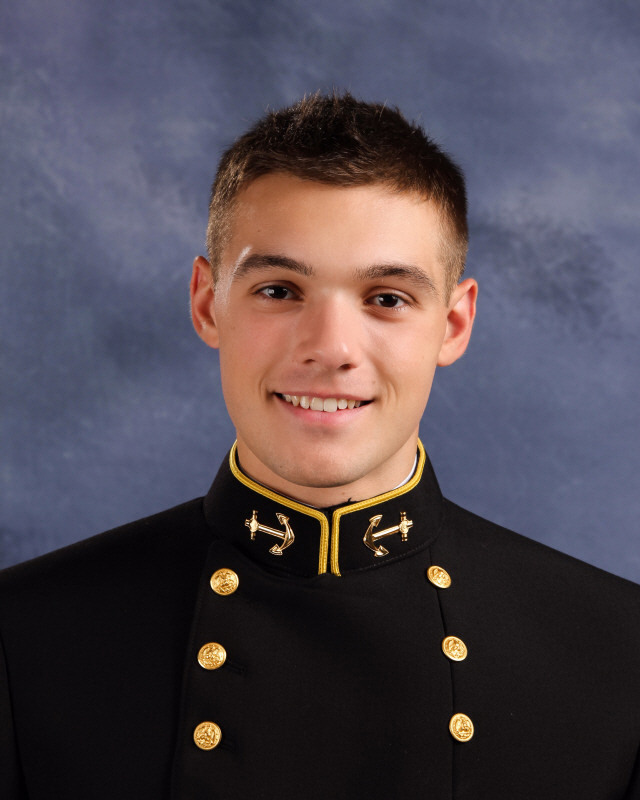
\includegraphics[width=1in,height=1.25in,clip,keepaspectratio]{\myroot/figures/M203876.jpg}}]{Ethan Marcello} is a midshipman at the United States Naval Academy majoring in Robotics and Control Engineering. Upon graduation, he hopes to service select Surface Warfare Officer with the Engineering Duty Officer option. 
%\end{IEEEbiography}
%
%\begin{IEEEbiography}[{
\includegraphics[width=1in,height=1.25in,clip,keepaspectratio]{\myroot/figures/evangelista_d_prof.jpg}}]{Dennis Evangelista} raises guide dog puppies. 
%\end{IEEEbiography}

\end{document}